%%
%% Customizações do abnTeX2 (http://abnTeX2.googlecode.com) para a Universidade XXXX
%%
%% This work may be distributed and/or modified under the
%% conditions of the LaTeX Project Public License, either version 1.3
%% of this license or (at your option) any later version.
%% The latest version of this license is in
%%   http://www.latex-project.org/lppl.txt
%% and version 1.3 or later is part of all distributions of LaTeX
%% version 2005/12/01 or later.
%%
%% This work has the LPPL maintenance status `maintained'.
%%
%% The Current Maintainer of this work is SEU_NOME, SEU_EMAIL
%%
%% Further information about abnTeX2 are available on https://github.com/abntex/abntex2
%%

% ---
% INICIO DAS CUSTOMIZACOES PARA A FACULDADE UNB GAMA
% ---

\newcommand{\curso}[1]{\def\imprimircurso{#1}}

\newcommand{\palavraChaveUm}[1]{\def\imprimirpalavrachaveum{#1}}
\newcommand{\palavraChaveDois}[1]{\def\imprimirpalavrachavedois{#1}}

\newcommand{\cdu}[1]{\def\nomecdu{#1}}
\newcommand{\dataDaAprovacao}[1]{\def\imprimirdatadaaprovacao{#1}}

\newcommand{\membroConvidadoUm}[1]{\def\imprimirmembroconvidadoum{#1}}
\newcommand{\membroConvidadoDois}[1]{\def\imprimirmembroconvidadodois{#1}}

\newcommand\BackgroundPic{%
	\put(0,0){%
		\parbox[b][\paperheight]{\paperwidth}{%
			\vfill
			\centering
			
\includegraphics[width=\paperwidth,height=\paperheight,%
				keepaspectratio]{figuras/capa.eps}%
			\vfill
		}
	}
}

\renewcommand{\imprimircapa}{%
  \begin{capa}%
    \center
	\AddToShipoutPicture*{\BackgroundPic}

%	\begin{huge}
%		\textbf{\textsc{Trabalho de Conclusão de Curso}}
%	\end{huge}

    \vspace*{2.7in}
	{\textbf{\large\imprimirinstituicao}}
	\par
	{\textbf{\large\imprimircurso}}

	\vspace{0.5in}

    {\ABNTEXchapterfont\bfseries\LARGE\imprimirtitulo}
    \vspace*{\fill}

	\begin{flushright}
    	\textbf{{\large{Autor: \imprimirautor}}}
		\par
    	\textbf{{\large{Orientador: \imprimirorientador}}}
	\end{flushright}

    \vspace*{0.2in}
    \textbf{{\large\imprimirlocal}}
    \par
    \textbf{{\large\imprimirdata}}

    \vspace*{2.2in}
  \end{capa}
}

% ---
% FIM DAS CUSTOMIZACOES PARA A FACULDADE UNB GAMA
% ---

\newcommand\fibtree{
\begin{figure}[htb]
	\centering
	\begin{tikzpicture}
	[
		grow = down,
		edge from parent/.style = {draw, -latex},
		every node/.style = {font=\footnotesize},
		sloped,
		level 1/.style = {
			sibling distance = 3cm,
			level distance = 1.5cm
		},
		level 2/.style = {
			sibling distance = 1.5cm,
			level distance = 1.5cm
		},
		level 3/.style = {
			sibling distance = 1.5cm,
			level distance = 1.5cm
		},
		level 4/.style = {
			sibling distance = 1.5cm,
			level distance = 1.5cm
		}
	]
		\node (1) { $F_n$ }
		child {	node (2) { $F_{n-1}$ }
		{
			child { node (3) { $F_{n-2}$ }
			{
				child { node (8) { $F_{n-3}$ } }
				child { node (9) { $F_{n-4}$ } }
			}}
			child {	node (4) { $F_{n-3}$ } }
		}}
		child { node (5) { $F_{n-2}$ }
		{
			child {	node (6) { $F_{n-3}$ } }
			child {	node (7) { $F_{n-4}$ } }
		}};

	\pgfsetfillopacity{0.1}
		\draw ($(3.north)+(0,0.5)$) -- (8.south west) -- (9.south east) -- cycle;
		\draw[dashed] ($(5.north)+(0,0.5)$) -- (6.south west) -- (7.south east) -- cycle;
%		\fill[fill=black] ($(3.north)+(0,0.5)$) -- (8.south west) -- (9.south east) -- cycle;
%		\draw[dashed] ($(5.north)+(0,0.5)$) -- (6.south west) -- (7.south east) -- cycle;
%		\draw ($(5.south west)-(0,0)$) -- ($(5.north east)+(0,0)$);
%		\draw ($(6.south west)-(0,0)$) -- ($(6.north east)+(0,0)$);
%		\draw ($(7.south west)-(0,0)$) -- ($(7.north east)+(0,0)$);
	\end{tikzpicture}
	\caption{Árvore de Fibonacci em P.D.}
	\label{fig:fib_tree}
\end{figure}
}

\newcommand\nimtree{
\begin{figure}[htb]
	\centering
	\begin{tikzpicture}
	[
		grow = down,
		edge from parent/.style = {draw, -latex},
		every node/.style = {font=\footnotesize},
		sloped,
		level 1/.style = {
			sibling distance = 5.9cm,
			level distance = 1.5cm
		},
		level 2/.style = {
			sibling distance = 2.4cm,
			level distance = 1.5cm
		},
		level 3/.style = {
			sibling distance = 1.5cm,
			level distance = 1.5cm
		},
		level 4/.style = {
			sibling distance = 1.5cm,
			level distance = 1.5cm
		}
	]
	\draw (-9,0) node {$J_1$};
	\draw [->][thick] (-8,0) -- (-7,0);
	\draw (-9,-1.5) node {$J_2$};
	\draw [->][thick] (-8,-1.5) -- (-7,-1.5);
	\draw (-9,-3) node {$J_1$};
	\draw [->][thick] (-8,-3) -- (-7,-3);
	\draw (-9,-4.5) node {$J_2$};
	\draw [->][thick] (-8,-4.5) -- (-7,-4.5);
	\draw (-9,-6) node {$J_1$};
	\draw [->][thick] (-8,-6) -- (-7,-6);
	\node (1) { $A$
		\begin{tikzpicture} {
			\draw (0,0) rectangle (1,0.7);
			\draw
			(0.15,0.15) -- (0.15,0.55)
			(0.3 ,0.15) -- (0.3 ,0.55)
			(0.7 ,0.15) -- (0.7 ,0.55)
			(0.85,0.15) -- (0.85,0.55);
		} \end{tikzpicture}
	}
	child {
		node (2) { $B$
			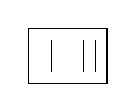
\begin{tikzpicture} {
				\draw (0,0) rectangle (1,0.7);
				\draw
				(0.3 ,0.15) -- (0.3 ,0.55)
				(0.7 ,0.15) -- (0.7 ,0.55)
				(0.85,0.15) -- (0.85,0.55);
			} \end{tikzpicture}} {
			child {
				node (4) { $D$
					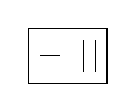
\begin{tikzpicture} {
						\draw (0,0) rectangle (1,0.7);
						\draw
						(0.15,0.35) -- (0.4 ,0.35)
						(0.7 ,0.15) -- (0.7 ,0.55)
						(0.85,0.15) -- (0.85,0.55);
					} \end{tikzpicture}}
				child {
					node (9) { $I$
					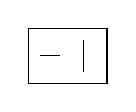
\begin{tikzpicture} {
						\draw (0,0) rectangle (1,0.7);
						\draw
						(0.15,0.35) -- (0.4,0.35)
						(0.7 ,0.15) -- (0.7,0.55);
					} \end{tikzpicture}
					}
					child {
						node (14) { $N$
							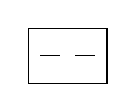
\begin{tikzpicture} {
								\draw (0,0) rectangle (1,0.7);
								\draw
								(0.15,0.35) -- (0.4 ,0.35)
								(0.6 ,0.35) -- (0.85,0.35);
							} \end{tikzpicture}
						}
					}
				}
				child {
					node (10) { $J$
						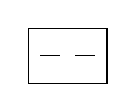
\begin{tikzpicture} {
							\draw (0,0) rectangle (1,0.7);
							\draw
							(0.15,0.35) -- (0.4 ,0.35)
							(0.6 ,0.35) -- (0.85,0.35);
						} \end{tikzpicture}
					}
				}
			}
			child {
				node (5) { $E$
					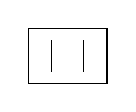
\begin{tikzpicture} {
						\draw (0,0) rectangle (1,0.7);
						\draw
						(0.3,0.15) -- (0.3,0.55)
						(0.7,0.15) -- (0.7,0.55);
					} \end{tikzpicture}
				}
				child {
					node (11) { $K$
						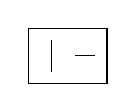
\begin{tikzpicture} {
							\draw (0,0) rectangle (1,0.7);
							\draw
							(0.3 ,0.15) -- (0.3 ,0.55)
							(0.6 ,0.35) -- (0.85,0.35);
						} \end{tikzpicture}
					}
					child {
						node (15) { $O$
							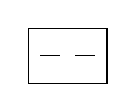
\begin{tikzpicture} {
								\draw (0,0) rectangle (1,0.7);
								\draw
								(0.15,0.35) -- (0.4 ,0.35)
								(0.6 ,0.35) -- (0.85,0.35);
							} \end{tikzpicture}
						}
					}
				}
			}
			child {
				node (6) { $F$
					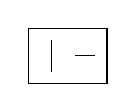
\begin{tikzpicture} {
						\draw (0,0) rectangle (1,0.7);
						\draw
						(0.3 ,0.15) -- (0.3 ,0.55)
						(0.6 ,0.35) -- (0.85,0.35);
					} \end{tikzpicture}
				}
				child {
					node (12) { $L$
						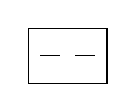
\begin{tikzpicture} {
							\draw (0,0) rectangle (1,0.7);
							\draw
							(0.15,0.35) -- (0.4 ,0.35)
							(0.6 ,0.35) -- (0.85,0.35);
						} \end{tikzpicture}
					}
				}
			}
		}
	}
	child {
		node (3) { $C$
			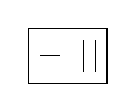
\begin{tikzpicture} {
				\draw (0,0) rectangle (1,0.7);
				\draw
				(0.15,0.35) -- (0.4 ,0.35)
				(0.7 ,0.15) -- (0.7 ,0.55)
				(0.85,0.15) -- (0.85,0.55);
			} \end{tikzpicture}
		} {
			child {
				node (7) { $G$
					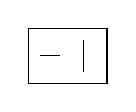
\begin{tikzpicture} {
						\draw (0,0) rectangle (1,0.7);
						\draw
						(0.15,0.35) -- (0.4 ,0.35)
						(0.7 ,0.15) -- (0.7 ,0.55);
					} \end{tikzpicture}
				}
				child {
					node (13) { $M$
						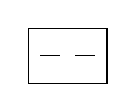
\begin{tikzpicture} {
							\draw (0,0) rectangle (1,0.7);
							\draw
							(0.15,0.35) -- (0.4 ,0.35)
							(0.6 ,0.35) -- (0.85,0.35);
						} \end{tikzpicture}
					}
				}
			}
			child {
				node (8) { $H$
					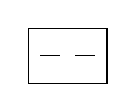
\begin{tikzpicture} {
						\draw (0,0) rectangle (1,0.7);
						\draw
						(0.15,0.35) -- (0.4 ,0.35)
						(0.6 ,0.35) -- (0.85,0.35);
					} \end{tikzpicture}
				}
			}
		}
	};
	\draw ($(14.south west)+(-1,-0.6)$) node {Vencedor:};
	\draw ($(14.south west)+(1.1,-0.6)$) node {($J_1$)};
	\draw ($(14.south west)+(2.6,-0.6)$) node {($J_2$)};
	\draw ($(14.south west)+(4.2,-0.6)$) node {($J_1$)};
	\draw ($(14.south west)+(6.6,-0.6)$) node {($J_2$)};
	\draw ($(14.south west)+(8.9,-0.6)$) node {($J_2$)};
	\draw ($(14.south west)+(11.2,-0.6)$) node {($J_1$)};
	\end{tikzpicture}
	\caption{Árvore do jogo \textit{Nim}}
	\label{fig:nim_tree}
\end{figure}
}
